% Author: Izaak Neutelings (July 2021)
% Description: ttbar jets
\documentclass[border=3pt,tikz]{standalone}
\usepackage{amsmath}
\usepackage{physics}
\usepackage{xcolor}
\usetikzlibrary{calc}
\usetikzlibrary{math} % for \tikzmath
\tikzset{>=latex} % for LaTeX arrow head
\usetikzlibrary{decorations.pathreplacing} % for curly braces

\colorlet{myblue}{blue!70!black}
\colorlet{mydarkblue}{blue!40!black}
\colorlet{mygreen}{green!80!black}
\colorlet{myred}{red!65!black}
\tikzstyle{vector}=[->,very thick,myblue,line cap=round]
\tikzstyle{ptmiss}=[->,dashed,thick,myred,line cap=round]
\tikzstyle{cone}=[thin,blue!50!black,fill=blue!50!black!30] %,fill opacity=0.8
\tikzstyle{conebase}=[cone,fill=blue!50!black!50] %,fill opacity=0.8

\newcommand\jetcone[5][blue]{{
  \pgfmathanglebetweenpoints{\pgfpointanchor{#2}{center}}{\pgfpointanchor{#3}{center}}
  \edef\ang{#4/2}
  \edef\e{#5}
  \edef\vang{\pgfmathresult} % angle of vector OV
  \tikzmath{
    coordinate \C;
    \C = (#2)-(#3);
    \x = veclen(\Cx,\Cy)*\e*sin(\ang)^2; % x coordinate P
    \y = tan(\ang)*(veclen(\Cx,\Cy)-\x); % y coordinate P
    \a = veclen(\Cx,\Cy)*sqrt(\e)*sin(\ang); % vertical radius
    \b = veclen(\Cx,\Cy)*tan(\ang)*sqrt(1-\e*sin(\ang)^2); % horizontal radius
    \angb = acos(sqrt(\e)*sin(\ang)); % angle of P in ellipse
  }
  \coordinate (tmpL) at ($(#3)-(\vang:\x pt)+(\vang+90:\y pt)$); % tangency
  \draw[thin,#1!40!black,rotate=\vang, %,fill=#1!50!black!80
    top color=#1!50!black!80,bottom color=#1!40!black!80,shading angle=\vang]
    (#3) ellipse({\a pt} and {\b pt});
  \draw[thin,#1!40!black,rotate=\vang,%fill=#1!80!black!40,
  top color=#1!90!black!20,bottom color=#1!50!black!50,shading angle=\vang]
    (tmpL) arc(180-\angb:180+\angb:{\a pt} and {\b pt})
    -- ($(#2)+(\vang:0.018)$) -- cycle;
}}


\begin{document}


% TTBAR JETS 
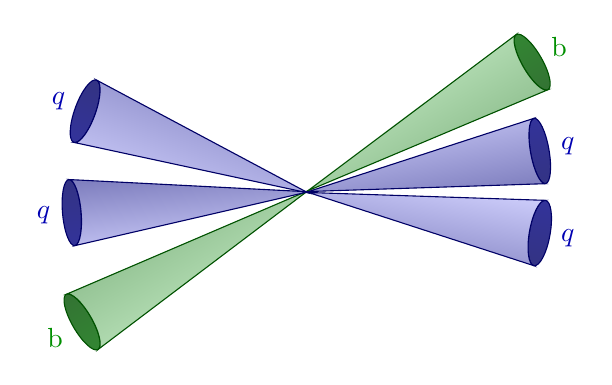
\begin{tikzpicture}
  \def\R{3}
  \coordinate (O) at (0,0);
  \coordinate (B1) at (  30:1.1*\R); % b jet 1
  \coordinate (J1) at (  10:1.0*\R); % q jet 1
  \coordinate (J2) at ( -10:1.0*\R); % q jet 2
  \coordinate (B2) at (-150:1.1*\R); % b jet 2
  \coordinate (J3) at ( 185:1.0*\R); % q jet 3
  \coordinate (J4) at ( 160:1.0*\R); % q jet 4
  
  % TOP 1
  \jetcone[mygreen]{O}{B1}{14}{0.10}
  \jetcone{O}{J1}{16}{0.08}
  \jetcone{O}{J2}{16}{0.10}
  \node[mygreen!70!black] at ($(O)!1.12!(B1)$) {b};
  \node[myblue] at ($(O)!1.12!(J1)$) {$q$};
  \node[myblue] at ($(O)!1.12!(J2)$) {$q$};
  %\draw[dashed] ($(O)!0.99!($(B1)!0.5!(J2)$)$) ellipse ({0.23*\R} and {0.62*\R});
  %\draw[dashed] ($(O)!0.5!($(B1)!0.5!(J2)$)$) arc(90:-90:{0.23*\R} and {0.62*\R});
  
  % TOP 2
  \jetcone[mygreen]{O}{B2}{14}{0.10}
  \jetcone{O}{J3}{16}{0.08}
  \jetcone{O}{J4}{16}{0.10}
  \node[mygreen!70!black] at ($(O)!1.12!(B2)$) {b};
  \node[myblue] at ($(O)!1.12!(J3)$) {$q$};
  \node[myblue] at ($(O)!1.12!(J4)$) {$q$};
  
\end{tikzpicture}


% TTBAR JETS - RECOILING 
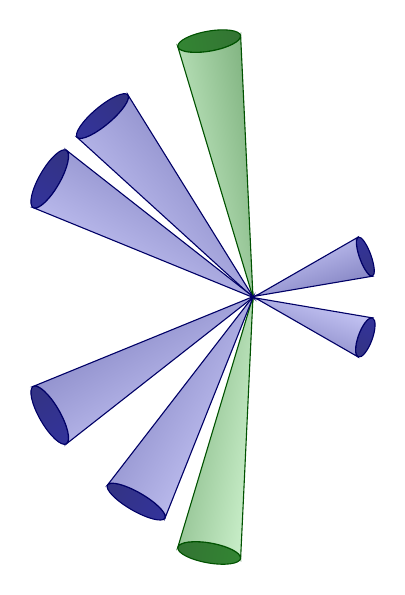
\begin{tikzpicture}
  \def\R{3}
  \coordinate (O) at (0,0);
  \coordinate (B1) at ( 100:1.1*\R); % b jet 1
  \coordinate (J1) at ( 130:1.0*\R); % q jet 1
  \coordinate (J2) at ( 150:1.0*\R); % q jet 2
  \coordinate (B2) at (-100:1.1*\R); % b jet 2
  \coordinate (J3) at (-120:1.0*\R); % q jet 3
  \coordinate (J4) at (-150:1.0*\R); % q jet 4
  \coordinate (R1) at (  20:0.5*\R); % recoil jet 1
  \coordinate (R2) at ( -20:0.5*\R); % recoil jet 2
  
  % TOP 1
  \jetcone[mygreen]{O}{B1}{14}{0.10}
  \jetcone{O}{J1}{16}{0.08}
  \jetcone{O}{J2}{16}{0.10}
  
  % TOP 2
  \jetcone[mygreen]{O}{B2}{14}{0.10}
  \jetcone{O}{J3}{16}{0.08}
  \jetcone{O}{J4}{16}{0.10}
  
  % RECOIL
  \jetcone{O}{R1}{20}{0.08}
  \jetcone{O}{R2}{20}{0.12}
  
\end{tikzpicture}



\end{document}